
% !TeX program = lualatex
% !TeX encoding = utf8
% !TeX spellcheck = uk_UA

\documentclass[]{article}
\usepackage{ds}
\addbibresource{SVM.bib}


\title{\sffamily\bfseries Метод опорних векторів}
\author{}
\date{}



\begin{document}
\maketitle

\begin{defbox}{Означення}
Метод опорних векторів (Support Vector Machine, SVM) --- це алгоритм машинного навчання для класифікації та регресії, який працює шляхом знаходження гіперплощини, що найкраще розділяє два або більше класи даних.
\end{defbox}

\section{Суть методу}

У SVM дані представляються у вигляді векторів у
$n$-вимірному просторі (де $n$ --- кількість ознак у даних), і для розділення класів шукається гіперплощина (тобто  ($n - 1$)-вимірна площина у  $n$-вимірному просторі), що максимально відділяє класи один від одного.

\begin{wrapfigure}[13]{l}{0.4\linewidth}\centering
	\begin{tikzpicture}[>=latex, scale=1.3]

		\coordinate (O) at (0.75, 1.1);

		\draw[->] (O) -- ++(4, 0) node[below right] {$x_1$};
		\draw[->] (O) -- ++(0, 4) node[left] {$x_2$};


		% Создаем два класса точек с разными цветами
		\foreach[count=\i] \x/\y in {
				1.1/3.4,
				1.1/2.6,
				1.1/4.0,
				1.5/3.5,
				1.6/3.1,
				1.8/2.5,
				2.0/3.6,
				2.0/4.3,
				2.4/4.0,
				2.6/3.3
			} {
                \node[circle, fill=blue, inner sep=2pt] (C\i) at (\x,\y) {};
                \draw[->, blue] (O) -- (C\i);
			}

		\foreach[count=\i] \x/\y in {
				2.9/1.5,
				3.3/2.3,
				3.3/1.6,
				3.6/1.4,
				3.6/1.9,
				4.1/2.4,
				4.1/1.7,
				4.4/1.4,
				4.6/2.3
			} {
                \node[circle, fill=green!50!black, inner sep=2pt] (C\i) at (\x,\y) {};
                \draw[->, green!50!black] (O) -- (C\i) ;
			}


		\begin{scope}[rotate=45]
			\draw[red] (1, -0.1) -- ++(6,0) node[above, rotate=45, pos=0.8] {гіперплощина};
		\end{scope}
	\end{tikzpicture}

    \caption{Ілюстрація суті методу опорних векторів}
\end{wrapfigure}

Оскільки може бути декілька таких гіперплощин, то SVM знаходить ту, яка максимізує мінімальну відстань між гіперплощиною та найближчими до неї точками обох класів (це відстань називається <<мінімальною шириною розділяючої смуги>> або <<margin>>).

SVM може використовуватися для класифікації даних, які мають два або більше класів, а також для регресії, тобто для передбачення числового значення залежної змінної на основі інших ознак даних. SVM є потужним алгоритмом машинного навчання, що зазвичай дає дуже хороші результати для класифікації даних у випадку, коли класи добре розділені гіперплощиною.

\section{Математична модель}

\subsection{Жорстке розділення}

\begin{defbox}{Означення}
Жорстке розділення (або hard margin) --- це концепція, яка описує ситуацію, коли алгоритм SVM прагне знайти таку гіперплощину (межу), яка повністю розділяє два класи даних без помилок.
\end{defbox}

\begin{figure}[h!]\centering
	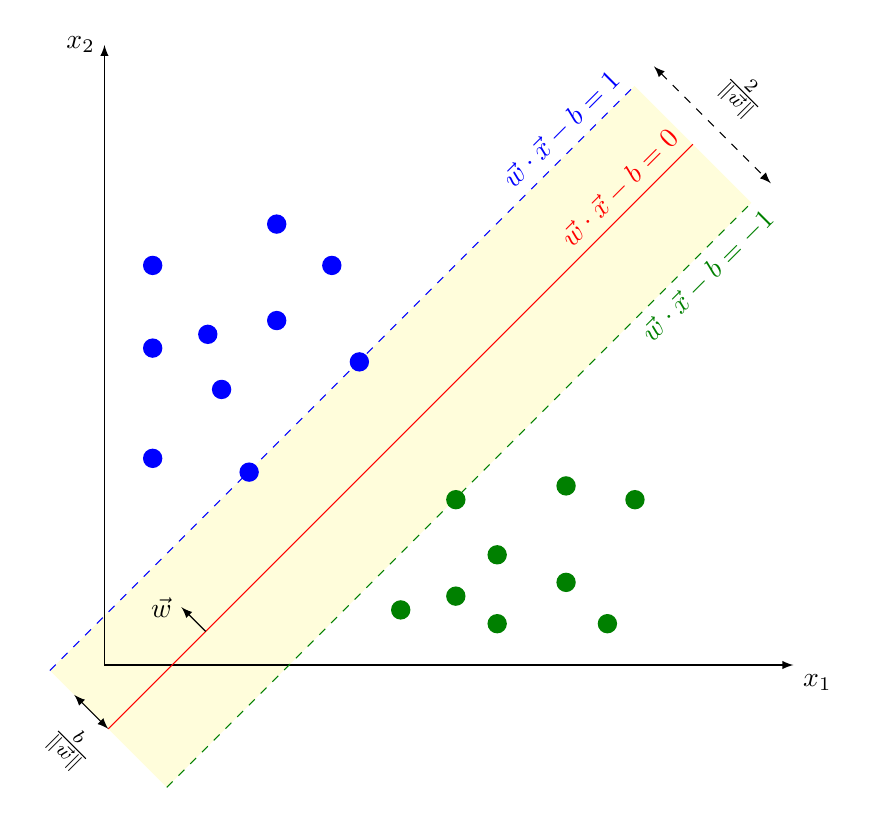
\begin{tikzpicture}[>=latex, scale=1.75]

		\coordinate (O) at (0.75, 1.1);

		\fill[rotate=45, yellow!20, opacity=0.7] (1, -0.7) rectangle ++(6,1.2);
		\draw[->] (O) -- ++(5, 0) node[below right] {$x_1$};
		\draw[->] (O) -- ++(0, 4.5) node[left] {$x_2$};


		% Создаем два класса точек с разными цветами
		\foreach \x/\y in {
				1.1/3.4,
				1.1/2.6,
				1.1/4.0,
				1.5/3.5,
				1.6/3.1,
				1.8/2.5,
				2.0/3.6,
				2.0/4.3,
				2.4/4.0,
				2.6/3.3
			} {
				\fill[blue] (\x,\y) circle (2pt);
			}

		\foreach \x/\y in {
				2.9/1.5,
				3.3/2.3,
				3.3/1.6,
				3.6/1.4,
				3.6/1.9,
				4.1/2.4,
				4.1/1.7,
				4.4/1.4,
				4.6/2.3
			} {
				\fill[green!50!black] (\x,\y) circle (2pt)
				% node[above, font=\tiny] {(\x, \y)}
				;
			}


		\begin{scope}[rotate=45]
			\draw[dashed, blue] (1, 0.5) --  ++(6,0) node[above, rotate=45, pos=0.9] {$\vec{w} \cdot \vec{x} - b = 1$};

			\draw[dashed, green!50!black] (1, -0.7) -- ++(6,0) node[below, rotate=45, pos=0.9] {$\vec{w} \cdot \vec{x} - b = -1$};

			\draw[red] (1, -0.1) -- ++(6,0) node[above, rotate=45, pos=0.9] {$\vec{w} \cdot \vec{x} - b = 0$};

			\draw[<->, dashed] (7.2, 0.5) -- (7.2, -0.7) node[pos=0.5,  rotate=-45, above=5pt] {$\frac2{\| \vec{w} \|}$};

			\draw[<->] (1, 0.25) -- (1, {(0.5-0.7)/2}) node[below=5pt, pos=0.5,  rotate=-45] {$\frac{b}{\| \vec{w} \|}$};

			\draw[black, ->] (2, {(0.5-0.7)/2}) -- ++(0, 0.25) node[left] {$\vec{w}$};
		\end{scope}
	\end{tikzpicture}
    \caption{Ілюстрація методу опорних векторів}
\end{figure}


Сформулюємо попереднє визначення більш строго та математично. В своїй основі ми маємо знову лінійну модель, і позначення ми використовуємо як і в попередніх модулях.

В нас є тренувальний набір даних з $n$ точок вигляду $ (\vec{x}_1, y_1),\, \ldots ,\, (\vec{x}_n, y_n) $, де $y_i$ є або $1$, або $-1$, і кожен з них вказує клас, до якого належить точка $\vec{x}_i$. Кожен $\vec{x}_i$  є $n$-вимірним вектором.

Нам треба знайти «максимально розділову гіперплощину», яка відділяє групу точок $\vec{x}_i$, для яких $y_i=1$, від групи точок, для яких $y_i=-1$, і визначається таким чином, що відстань між цією гіперплощиною та найближчою точкою $\vec{x}_i$ з кожної з груп є максимальною.

%Будь-яку гіперплощину може бути записано як множину точок $\vec{x}$, які задовольняють умові:
%\begin{equation*}
%    \vec{w}\cdot\vec{x} - b=0,
%\end{equation*}
%де $\vec{w}$ є (не обов'язково нормалізованим) до цієї гіперплощини.

Якщо тренувальні дані лінійно роздільні, то ми можемо обрати дві паралельні гіперплощини, які розділяють два класи даних так, що відстань між ними якомога більша. Область, обмежена цими двома гіперплощинами, називається «розділенням» (margin), а максимально розділова гіперплощина це гіперплощина, яка лежить посередині між цими двома. Ці гіперплощини може бути описано рівняннями:
\begin{align*}
    \vec{w}\cdot\vec{x} - b &= 1,\ \text{\small (будь-що на або вище цієї межі належить до класу з міткою $1$)} \\
    \vec{w}\cdot\vec{x} - b &= -1,\ \text{\small (будь-що на або вище цієї межі належить до класу з міткою $-1$)}
\end{align*}


Оскільки ми також маємо завадити потраплянню точок даних до розділення, ми додаємо таке обмеження:
\begin{equation}\label{eq:inequality}
	\begin{cases}
		\vec{w}\cdot \vec{x}^{(i)} - b \geqslant 1,  & \text{якщо}\ y^{(i)} = 1, \\
		\vec{w}\cdot \vec{x}^{(i)} - b \leqslant -1, & \text{якщо}\ y^{(i)} = -1
	\end{cases}
\end{equation}

Ці обмеження стверджують, що кожна точка даних мусить лежати з правильного боку розділення.

Таке розділення класів гіперплощиною називається жорстким, оскільки така модель не дозволяє робити помилок, і різні класи чітко лежать по різні сторони гіперплощини, що розділяє класи. Геометрично ширина смуги, що розділяє класи (margin) дорівнює
$\dfrac2{\|\vec{w}\|}$, де $\|\vec{w}\|$ норма вектору вагових коефіцієнтів, що рівна кореню зі скалярного добутку вектора вагових коефіцієнтів самого на себе, тобто:
\begin{equation*}
	\|\vec{w}\| = \sqrt{\vec{w}\cdot \vec{w} } = \sqrt{\sum_{i=1}^n w_i^2}.
\end{equation*}

І оскільки ми хочемо максимізумати ширину розділяючої смуги:

\begin{equation*}
    \dfrac2{\|\vec{w}\|} \to \max,
\end{equation*}
то такий тип класифікаторів називають maximum margin.

В свою чергу, проблема знаходження максимуму еквівалентна до проблеми знаходження мінімуму:

\begin{equation*}
   \|\vec{w}\|^2 \to \min,
\end{equation*}
тобто величина норми вектора вагових коефіцієнтів повинна бути мінімальною. А тому, ми можемо привести цю задачу до оптимізаційної і використати алгоритм градієнтного спуску та знайти оптимальні значення коефіцієнтів~$w_i$\footnote{Зауважимо, що останнє визначення довжини вектору може нам дещо нагадати --- а саме доданок $L_2$-регуляризації.}.



\subsection{М'яке розділення}

Жорстке розділення --- це ідеальна ситуація, в реальних даних жорстке розділення може бути неможливим через наявність шуму або перекриття класів.

\begin{defbox}{Означення}
Для задач, у яких дані не можна жорстко розділити, використовують гнучкіший метод, який називають м'яким розділенням (soft margin), що дає змогу деяким об'єктам перебувати на <<неправильній>> стороні межі з певною помилкою, але водночас намагається мінімізувати цю помилку й забезпечити найкраще розділення класів.
\end{defbox}

%При жорсткому розділенні модель не дозволяє робити помилок. Проте у наших даних можуть бути якісь аномалії, чи неправильно розмічені приклади, в такому випадку якщо ми будемо спиратись на такі дані, модель навчиться неоптимально, і буде дуже чутлива до таких аномалій.

%Щоб уникнути цього ми

Дозволимо нашому класифікатору робити помилки, проте нам потрібно оцінити наскільки сильно помиляється класифікатор і додати ці оцінки у функцію втрат.

Спочатку вияснимо, як порахувати такі оцінки.

Нерівності~\eqref{eq:inequality} можна переписати в одну:
\begin{equation}\label{eq:integrateg_ineq}
    y_i \left[ \vec{w}\cdot \vec{x}^{(i)} - b \right] \geqslant 1
\end{equation}

Нам необхідно придумати таку функцію, яка дорівнює $0$, якщо обмеження в \eqref{eq:integrateg_ineq} задовольняється, іншими словами, якщо $x_i$
лежить із правильного боку розділення. Для даних із неправильного боку розділення значення цієї функції є пропорційним до відстані $M_i$ від розділення. Ця відстань дорівнює  $M_i = y_i \left[ \vec{w}\cdot \vec{x}^{(i)} - b \right]$. В результаті ми отримаємо таку функцію втрат:

\def\mo{\max\left(0, 1 - y_i \left[ \vec{w}\cdot \vec{x}^{(i)} - b \right]\right)}
\def\mt{\max\left(0, 1 + y_i \left[ \vec{w}\cdot \vec{x}^{(i)} - b \right]\right)}

\begin{equation}
		 \mo
\end{equation}

Ця функція називається завісною функцією втрат (англ. hinge loss function).

Отже, повна функція втрат :
\begin{equation}
	\mathrm{Loss} = \frac1{m} \sum_{i = 1}^m \mo + \lambda \|\vec{w}\|^2
\end{equation}
де параметр $\lambda$ визначає компроміс між збільшенням розміру розділення та забезпеченням того, що $x_i$ лежить із правильного боку розділення. Таким чином, для достатньо малих значень $\lambda$ SVM із м'яким розділенням поводитиметься однаково з SVM із жорстким розділенням, якщо вхідні дані є лінійно класифіковними.

Поглянемо на графіки й порівняємо функцію втрат для логістичної регресії та методу опорних векторів~(рис.~\ref{comparison}).


\begin{figure}[htbp!]
	\centering
%	\subcaptionbox{}
%	{
    \begin{tikzpicture}[trim left]
			\begin{axis}[
					width=0.75\linewidth,
					height=0.65\linewidth,
					xlabel=Значення параметра,
					ylabel=$\mathrm{Loss}$,
					grid=both,
					y label style={at={(axis description cs:0, 0.5)},anchor=north},
					xtick distance = 1,
					ytick distance = 1,
					xticklabel style={font=\footnotesize},
					yticklabel style={font=\footnotesize},
					legend style={opacity=0.75},
				]

				% График для логистической регрессии
				\addplot[color=blue,mark=none,smooth] {ln(1 + exp(-x)};
				\addlegendentry{Логістична регресія}

				% График для метода опорных векторов
				\addplot[color=red,mark=none,smooth, samples=1000] {max(0, 1 - x)};
				\addlegendentry{Hinge Loss}

			\end{axis}
		\end{tikzpicture}
%        }
%	\subcaptionbox{}
%	{\begin{tikzpicture}
%			\begin{axis}[
%					width=0.5\linewidth,
%					height=0.45\linewidth,
%					xlabel=Значення параметра,
%					ylabel=$\mathrm{Loss}$,
%					grid=both,
%					y label style={at={(axis description cs:0, 0.5)},anchor=north},
%					xtick distance = 1,
%					ytick distance = 1,
%					xticklabel style={font=\footnotesize},
%					yticklabel style={font=\footnotesize},
%					legend style={opacity=0.75},
%				]
%
%				% График для логистической регрессии
%				\addplot[color=blue,mark=none,smooth] {ln(1 + exp(x)};
%				\addlegendentry{Логістична регресія}
%
%				% График для метода опорных векторов
%				\addplot[color=red,mark=none,smooth, samples=1000] {max(0, 1 + x)};
%				\addlegendentry{SVM: $\mathrm{cost}_2$}
%
%			\end{axis}
%		\end{tikzpicture}}
	\caption{Порівняння функції втрат для логістичної регресії та методу опорних векторів}\label{comparison}
\end{figure}




\section{Ядровий трюк}

Ось ми розібрались, як побудувати лінійний класифікатор за допомогою методу опорних векторів. Проте, як ми знаємо, часто ми не можемо лінійно розділити наші дані, як наприклад на ілюстрації~\ref{fig:inseparable}.

Для цього ми повинні перейти до нового простору ознак, раніше ми займались створенням нових фіч, таких як $x_j^2$ чи $x_j^3$, у такому випадку ми повинні перевести всі наші дані у новий векторний простір доповнений новими штучно створеними ознаками. Та це може бути досить дорого з точки зору обчислень, а ядровий трюк полягає у тому, що ми не робимо трансформацію даних, щоб відобразити їх у новому векторному просторі, а лише розраховуємо відстані між векторами так, наче ми вже перебуваємо у цьому просторі.


\begin{wrapfigure}{l}{0.5\linewidth}
	\centering
	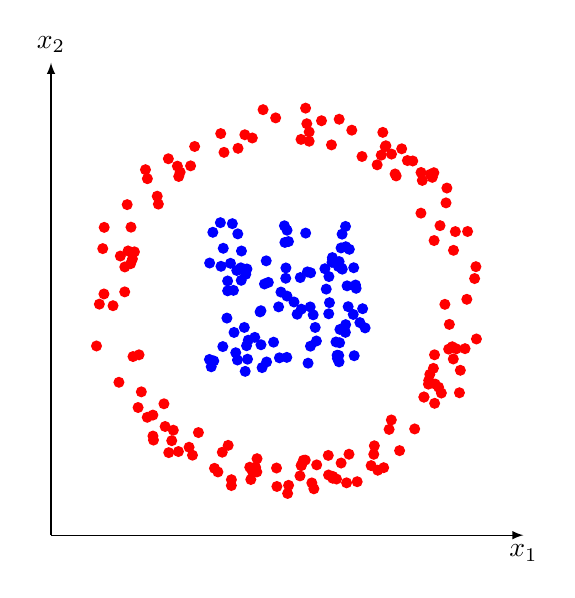
\begin{tikzpicture}[>=latex]

		% Класс 1 - внутренний круг
		\foreach \i in {1,...,100} {
				\pgfmathsetmacro{\x}{-1 + 2*rnd}
				\pgfmathsetmacro{\y}{-1 + 2*rnd}
				\fill[blue] (\x,\y) circle (2pt);
			}

		% Класс 2 - внешний круг
		\foreach \i in {1,...,150} {
				\pgfmathsetmacro{\angle}{rnd*360}
				\pgfmathsetmacro{\radius}{2 + rnd*0.5}
				\pgfmathsetmacro{\x}{\radius*cos(\angle)}
				\pgfmathsetmacro{\y}{\radius*sin(\angle)}
				\fill[red] (\x,\y) circle (2pt);
			}

		% Оси координат
		\draw[->] (-3,-3) -- ++(6,0) node[below] {$x_1$};
		\draw[->] (-3,-3) -- ++(0,6) node[above] {$x_2$};
	\end{tikzpicture}
	\caption[Не роздільні]{Не роздільні ознаки}
	\label{fig:inseparable}
\end{wrapfigure}
Це досягається за допомогою ядерної функції, яка обчислює скалярний добуток між векторами у вищорозмірному просторі, не потребуючи безпосереднього перетворення даних у цей простір. Це дозволяє SVM працювати зі складними нелінійно-роздільними даними, зберігаючи при цьому швидкість роботи алгоритму.

Застосування ядерного трюку в SVM дозволяє підвищити точність класифікації та зменшити ризик перенавчання моделі. Проблеми, які можуть бути вирішені за допомогою SVM з ядерним трюком, включають класифікацію текстових даних, розпізнавання образів та прогнозування фінансових показників.

Існує кілька типів ядерних функцій, які можна використовувати з методом опорних векторів (SVM), залежно від характеристик даних та завдання класифікації. Ось деякі з найпоширеніших ядерних функцій:

\begin{itemize}
	\item Лінійна функція ядра: $K(x, y) = xy$;
	\item Поліноміальна функція ядра: $K(x, y) = (xy + r)^d$, де $r$ --- константа зміщення. $d$ --- степінь полінома;
	\item Радіальна базисна функція (RBF) ядра: $K(x, y) = e^{-\gamma \cdot \|x - y\|^2}$, де $\gamma$ --- параметр ширини гаусівської функції;
	\item Сигмоїдальна функція ядра: $K(x, y) = \tanh(\alpha\cdot xy + r)$, де $\alpha$ ---  параметр швидкості зростання,  $r$ --- константа зміщення.
\end{itemize}

Кожен тип ядерної функції має свої унікальні властивості та може бути корисним для різних завдань класифікації. Наприклад, лінійна функція ядра добре підходить для лінійно роздільних даних, тоді як RBF функція може допомогти з розділенням складних нелінійних даних.

\subsection{Гаусівське ядро}

Розглянемо більш детально радіально базисну функцію, котра також називається ще й гаусівським ядром. Напишемо формулу густини ймовірності гаусівського розподілу:

\begin{equation*}
	f(x) = \frac1{\sqrt{2\pi}\sigma}e^{-\frac{(x - \mu)^2}{2\sigma^2}}.
\end{equation*}

Де символи $\mu$ та $\sigma$ позначають математичне очікування та стандартне відхилення відповідно. Тоді як ядрова функція радіального базису має такий вигляд:

\begin{equation*}
	K(x, y) = e^{-\gamma \cdot \|x - y\|^2}.
\end{equation*}

Ну і якщо ми зробимо такі заміну $\gamma = \dfrac1{2\sigma^2}$, то побачимо що дані функції відрізняються лише множенням на скаляр.

Проте як саме працює ядровий трюк? Як ми бачимо з визначенням ядрових функції в розрахунках ми використовуємо два вектори $\vec{x}$ та $\vec{y}$ і ми розраховуємо відстань між ними у новому лінійному просторі. А далі, у якості нових ознак для нашої моделі, описаної вище, ми будемо брати нові ознаки --- відстані між нашими приклади розраховані за допомогою нашої ядрової функції. Формалізуємо вище сказане твердження:

\begin{equation*}
	f_j^{(i)} = K(\vec{x}^{(i)}, \vec{x}^{(j)}) = e^{-\gamma \cdot \|\vec{x}^{(i)} - \vec{x}^{(j)}\|^2}.
\end{equation*}

Отже тепер ми маємо замість вектора $\vec{x}^{(i)} \in \mathbb{R}^n$ новий $f^{(i)} \in \mathbb{R}^m$. І тепер будемо використовувати нові ознаки і в новому просторі шукати розподільчу смугу і максимізувати її ширину.

\section{Реалізація методу SVM у бібліотеці \texttt{scikit-learn}}

Вся вищенавадена математична модель вже є реалізована у знайомій нам бібліотеці, і ви можете ознайомитись більше з різними версіями даного методу за \href{https://scikit-learn.org/stable/modules/svm.html}{посиланням}. А тут наведемо приклад використання SVM в елементарному прикладі:

\begin{minted}[bgcolor=lightgray!20, fontsize=\scriptsize]{python}
from sklearn import svm

X = [[0, 0], [1, 1]]
y = [0, 1]

clf = svm.SVC()
clf.fit(X, y)

print(clf.predict([[2., 2.]]))
\end{minted}


Або більш складніший приклад:

\begin{minted}[bgcolor=lightgray!20, fontsize=\scriptsize]{python}
# Import the necessary libraries
import numpy as np
import matplotlib.pyplot as plt
from sklearn import datasets
from sklearn.model_selection import train_test_split
from sklearn.svm import SVC

# Generate synthetic data (two point classes)
X, y = datasets.make_classification(
    n_samples=100,
    n_features=2,
    n_informative=2,
    n_redundant=0,
    n_clusters_per_class=1,
    random_state=42)

# Split the data into training and test sets
X_train, X_test, y_train, y_test = train_test_split(
    X, y, test_size=0.2, random_state=42)

# Create and train the SVM model
svm_classifier = SVC(kernel='linear', C=1)
svm_classifier.fit(X_train, y_train)

# Output the classification accuracy on the test set
accuracy = svm_classifier.score(X_test, y_test)
print(f'Classification accuracy: {accuracy:.2f}')

# Create a grid to visualize the solution boundary
xx, yy = np.meshgrid(np.linspace(X[:, 0].min() - 1,
                                 X[:, 0].max() + 1, 100),
                     np.linspace(X[:, 1].min() - 1,
                                 X[:, 1].max() + 1, 100))
Z = svm_classifier.decision_function(np.c_[xx.ravel(), yy.ravel()])
Z = Z.reshape(xx.shape)

# Data visualization and decision boundaries
plt.figure(figsize=(8, 6))
plt.contourf(xx, yy, Z,
             levels=[-1, 0, 1],
             colors=['r', 'g', 'b'], alpha=0.2)
plt.scatter(X[:, 0], X[:, 1], c=y,
            cmap=plt.cm.coolwarm,
            edgecolors='k')
plt.xlabel('Feature 1')
plt.ylabel('Feature 2')
plt.title('Reference vector method (SVM)')
plt.show()
\end{minted}


\section*{Висновок}

SVM (англ. Support Vector Machine) --- це метод машинного навчання, який знайшов широке застосування в задачах класифікації та регресії. Основною ідеєю методу є побудова гіперплощини, яка розділяє два класи даних з максимальною можливою шириною проміжку між ними.

При роботі з SVM ми спочатку перетворюємо наші дані до більш високої розмірності за допомогою ядерної функції, що дозволяє лінійно нероздільні дані перетворювати в лінійно роздільні. Потім ми побудовуємо гіперплощину, максимізуючи відстань між гіперплощиною і найближчими до неї точками (векторами опору). Ці точки називаються опорними векторами і вони є ключовими елементами моделі SVM.

Серед переваг методу SVM можна виділити високу точність класифікації в задачах з великою кількістю ознак та можливість використання різних ядерних функцій для перетворення даних, які підходять для різних типів даних та задач.

Однак, метод SVM може бути чутливий до викидів, тобто до даних, які значно відрізняються від інших даних у вибірці. Крім того, вибір оптимальних параметрів для SVM може бути часо- та ресурсомістким завданням.

У загальному, SVM є потужним та ефективним методом машинного навчання, який може бути застосований у багатьох різних задачах. Використання SVM може залежати від характеру даних та конкретних умов задачі, тому варто розглянути його як один з варіантів при вирішенні конкретної задачі.

\clearpage
\nocite{*}
\printbibliography[title=Посилання]


\end{document}


